%%%%%%%%%%%%%%%%%%%%%%%%%%%%%%%%%%%%%
% Document properties and packages
%%%%%%%%%%%%%%%%%%%%%%%%%%%%%%%%%%%%%
\documentclass[a4paper,12pt,final]{memoir}
\usepackage{CJKutf8}%中文支持
\usepackage{float}
% misc
\renewcommand{\familydefault}{bch}	% font
\pagestyle{empty}					% no pagenumbering
\setlength{\parindent}{0pt}			% no paragraph indentation
% required packages (add your own)
\usepackage{flowfram}% column layou
\usepackage{marvosym}
\usepackage{textcomp}

\usepackage[top=1cm,left=1cm,right=1cm,bottom=1cm]{geometry}% margins
\usepackage{graphicx}										% figures
\usepackage{hyperref}
\definecolor{linkcolour}{rgb}{0,0.2,0.6}  %蓝色
\hypersetup{colorlinks,breaklinks,urlcolor=linkcolour, linkcolor=linkcolour}										% URLs
\usepackage[usenames,dvipsnames]{xcolor}					% color
\usepackage{multicol}										% columns env.
	\setlength{\multicolsep}{0pt}
\usepackage{paralist}										% compact lists
\usepackage{tikz}

%%%%%%%%%%%%%%%%%%%%%%%%%%%%%%%%%%%%%
% Create column layout
%%%%%%%%%%%%%%%%%%%%%%%%%%%%%%%%%%%%%
% define length commands
\setlength{\vcolumnsep}{\baselineskip}
\setlength{\columnsep}{\vcolumnsep}
%定义主题颜色,可选颜色 Maroon,ForestGreen,DarkOrchid,RoyalBlue,Turquoise,Cyan,etc,更多颜色参考xcolor包的颜色定义
\newcommand{\myThemeColor}{RoyalBlue}
% frame setup (flowfram package)
% left frame
\newflowframe{0.23\textwidth}{\textheight}{0pt}{0pt}[left]
	\newlength{\LeftMainSep}
	\setlength{\LeftMainSep}{0.23\textwidth}
	\addtolength{\LeftMainSep}{1\columnsep}
 
% small static frame for the vertical line
\newstaticframe{1.5pt}{\textheight}{\LeftMainSep}{0pt}
 
% content of the static frame
\begin{staticcontents}{1} %绘制分割线,使用tikz包绘制。如需改变风格线样式,请参考tikz教程,对于新手,不建议修改。
\hfill
\tikz{%
	\draw[loosely dotted,color=\myThemeColor,line width=1.5pt,yshift=0]
	(0,0) -- (0,\textheight);}%
\hfill\mbox{}
\end{staticcontents}
 
% right frame
\addtolength{\LeftMainSep}{1.5pt}
\addtolength{\LeftMainSep}{1\columnsep}
\newflowframe{0.7\textwidth}{\textheight}{\LeftMainSep}{0pt}[main01]


%%%%%%%%%%%%%%%%%%%%%%%%%%%%%%%%%%%%%
% define macros (for convience)
%%%%%%%%%%%%%%%%%%%%%%%%%%%%%%%%%%%%%
\newcommand{\Sep}{\vspace{1em}}
\newcommand{\SmallSep}{\vspace{0.9em}}

\newenvironment{AboutMe}
	{\ignorespaces\textbf{\color{\myThemeColor} About me}}
	{\Sep\ignorespacesafterend}
%定义section	
\newcommand{\CVSection}[1]
	{\Large\textbf{#1}\par
	\vspace{0.2cm}\normalsize\normalfont}

\newcommand{\CVItem}[1]
	{\textbf{\color{\myThemeColor} #1}}


%%%%%%%%%%%%%%%%%%%%%%%%%%%%%%%%%%%%%
% Begin document
%%%%%%%%%%%%%%%%%%%%%%%%%%%%%%%%%%%%%
\begin{document}

\begin{CJK*}{UTF8}{gbsn}%选择字体,黑体
% Left frame 左边内容在此定义
%%%%%%%%%%%%%%%%%%%%
\begin{figure}
	\hfill
	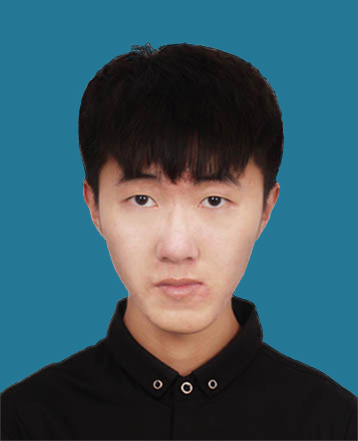
\includegraphics[width=0.8\columnwidth]{photo}
	\vspace{-7cm}
\end{figure}
\begin{flushright}\footnotesize
.\\
\vskip 6cm
    \raggedright
	\CVItem{{\large 个人信息:}}\\
	电子邮件:\\
	\href{mailto:jiafeng5513@163.com}{jiafeng5513@163.com}  \\
	Github:\\
	\href{github.com/jiafeng5513}{github.com/jiafeng5513} \\
	手机:\\
	15764356880
	\SmallSep
	\SmallSep

	\CVItem{{\large 求职意向:}}\\
	\textit{游戏开发,客户端或工具开发\\ }
	\SmallSep

	\CVItem{{\large 语言能力:}}\\
	\textit{\textbf{英语}:CET-6\\ }
	\SmallSep

	\CVItem{{\large 技能:}}\\
	$\bullet$\textbf{编程语言:}\\ C\#/C++/Java/Python\\
	$\bullet$\textbf{开发专长:}\\ 桌面客户端开发/图像处理/机器视觉 \\
	\SmallSep
	\textit{具备较丰富的桌面客户端,机器视觉和深度学习的开发经验,对U3D和UE4具有一定的使用经验,有较强的学习能力,具备英文文献查阅理解和写作能力.}
	
	% \CVItem{{\large 爱好:}}\\
	% \textit{视频制作,口琴,骑行}
	\SmallSep
	\SmallSep
	\SmallSep
	
	\CVItem{\large Link To My Github}
	\begin{figure}[h]
		\centering
		
\includegraphics[width=0.8\columnwidth]{Github.png}
	\end{figure}
	

\end{flushright}\normalsize
\framebreak


% Right frame 右边内容在此定义
%%%%%%%%%%%%%%%%%%%%
\Huge\bfseries {\color{\myThemeColor} 贾~~锋}\\
\normalsize\normalfont

% Education
\CVSection{教育背景}
\hrule
\SmallSep
\CVItem{2017 - 目前\hfill\textsc{Jilin University,吉林大学}}\\
\textit{-计算机科学与技术学院}\\
\textit{-计算机应用技术在读研究生}
\textit{-毕业时间:2020}
\\
\CVItem{2013 - 2017\hfill\textsc{Jilin University,吉林大学}}\\
\textit{-软件学院,专业排名21/251}\\
\textit{-学士学位}\\
\textit{-保研本校}\\

% CAMPU
\CVSection{专业经历}
\hrule
\SmallSep
\CVItem{本科毕业设计\hfill\emph{独立完成}}\\
\textit{$\bullet$ 基于Qt的神经网络辅助设计系统.设计并实现了用于支持深度学习的GUI程序,封装了Caffe的主要功能,为Caffe的使用提供语法高亮,参数含义指示等辅助功能.能使用UI直接进行深度模型的训练,能够切换Caffe源.进行了初步的可视化编程尝试.} 
\\
\CVItem{用于深度学习和图像处理的可视化编程环境 \hfill\emph{独立完成}}\\
\textit{$\bullet$ 基于本科毕业设计的主要思想,使用.NET WPF设计并实现了节点式的图形化编程环境,采用类似Unreal Engine 4引擎中蓝图脚本的UI设计,将图像处理和深度学习所需的操作封装成节点,供用户拖放式使用,能够即时得出运算结果.设计了轻量化扩展接口,用户无需了解本程序的内部实现,也无需重新编译本程序的源代码,即可向系统中添加自定义节点,实现任意功能.截止目前,内置节点已经涵盖了全部的算术运算以及大量的常用函数和操作,并能够组建普通卷积,残差等网络模型并进行训练和测试.目前已投稿Transactions on Visualization and Computer Graphics(JCR二区).}
\\
\CVItem{医学影像处理研究 \hfill\emph{参与研究}}\\
\textit{$\bullet$ 实验室项目.前期主要负责使用Qt/C++编写DICOM格式医学影像处理程序,实现医学影像的显示测量,分割,三维重建等功能.后期进行基于肺部CT影像肺癌辅助诊断研究,主要使用深度学习和传统图像处理方法,进行肺结节的定位与分类,阅读并重现了一些论文中的工作,并使用我自己开发的可视化编程环境设计了一套数据集标定流程,设计并实现了一个基于U-Net和Faster-Rcnn的肺结节检测分类系统,实现了98\%左右的检测准确率,目前该工作已经移交给他人.}
\\
\CVItem{开源项目\hfill\emph{项目负责人}}\\
\textit{$\bullet$ 原大创项目,后逐渐扩展为一个视觉算法实验平台,研究并实现双目视觉系统,负责全部代码的编写.项目使用C++开发,涉及双目摄像机的标定,匹配,三维重建,目标检测以及距离解算.提供多种视差算法备选,目前仍保持更新,有相关技术博客和资源.此外本人一直跟踪三维重建和相关视觉算法的进展.} 
\\

% HONORS & SCHOLARSHIPS
\CVSection{个人荣誉}
\hrule
\SmallSep
	\begin{tabular}{l|l}
		$\Rightarrow$ 本科期间&\textit{两次三等奖学金,两次一等奖学金,优秀毕业生}\footnotesize\\
		$\Rightarrow$ 硕士期间&\textit{入学奖学金}\\
	\end{tabular}

%%%%%%%%%%%%%%%%%%%%%%%%%%%%%%%%%%%%%
% End document
%%%%%%%%%%%%%%%%%%%%%%%%%%%%%%%%%%%%%
\end{CJK*}
\end{document}